\documentclass[12pt,letterpaper]{hmcpset}
\usepackage[margin=1in]{geometry}
\usepackage{graphicx}
\usepackage{hyperref}

% info for header block in upper right hand corner
\name{Name: \underline{\hspace{4cm}}}
\class{Math 45: Section \underline{\hspace{1cm}}}
\assignment{Assignment 2}
\duedate{3/23/18}

\begin{document}


\begin{problem}
1. (5 points) Complex numbers are helpful when expressing oscillatory behavior using trigonometric
functions. Euler’s formula helps us to convert from complex exponentials like $e^{i\theta}$ to
trigonometric functions like cosine and sine:
\begin{center}
$e^{i\theta} = cos(\theta) + isin(\theta)$.    
\end{center}
How do we convert from cosine and sine into complex exponentials? Consider that
\begin{center}
$e^{-i\theta} = cos(-\theta) + isin(-\theta)=cos(\theta) - isin(\theta)$.    
\end{center}
Add the two equations above and solve for $cos(\theta)$. Subtract to solve for $sin(\theta)$.\\
\textbf{Recall} that $i$ is used to represent the number $\sqrt{-1}$ and that $i^2 = -1$.
\end{problem}
\newpage

\begin{problem}
2. (5 points) Simplify each of the following expressions, assuming that $a$, $t$, $\omega$ are real numbers.\\
Example:  Re($e^{i\omega t}$) $=$ Re [$cos(\omega t) + isin(\omega t)$] $=$ $cos(\omega t)$

\begin{enumerate}
    \item[(a)] Im($e^{i\omega t}$)= 
    \item[(b)] Re($e^{-i\omega t}$)= 
    \item[(c)] Re($e^{(a+i\omega) t}$)=Re($e^{at}e^{i\omega t}$)=Re[$e^{at}cos(\omega t) + ie^{at}isin(\omega t)$]$=$ 
    \item[(d)] Im($e^{(a+i\omega) t}$) =
\end{enumerate}

\end{problem}
\newpage

\begin{problem}
3. (5 points) For each of the following ordinary differential equations, indicate its order, whether
it is autonomous or non-autonomous, whether it is linear or nonlinear, and whether it is
driven or undriven.\\

\begin{enumerate}
    \item[(a)] $ \frac{dg}{dx}+g^3=0$
    \item[(b)] $\ddot{y}(t)+e^{ty(t)}=cosh(t)$ \textbf{Note:} $\ddot{y}(t)$is the same as $y''(t)= \frac{d^2 y}{dt^2}$ 
    \item[(c)] $r^2R''(r) + rR'(r)-5R(r) =0$
    \item[(d)] $\ddot{\theta}+sin(\theta)=0$
    \item[(e)] $f'''=f'+xf+4sin(x)$
    \item[(f)] $\frac{y'}{y}=7$ \textbf{Note:} If possible, rewrite this DE so that it is linear. If not, explain why.
\end{enumerate}

\end{problem}
\newpage


\begin{problem}
4. (10 points total: 5 points for tasks 1 \& 2, 5 points for task 3) (Problem from Floyd Bullard,
NCSSM) In this problem you will simulate fishing from a stocked pond using dice simulated
in R. If you don’t want to use R, you can use a dice rolling program like the number (integer)
generator at random.org. You might want to sort and count the results in a spreadsheet.\\\\
Scenario: A community has a pond that is stocked with 10, 000 fish annually. People fish
throughout the year, catching fish at a rate proportional to how many fish are in the pond,
with the proportionality constant being about 1/6 per year. At time t = 0 there are 15, 000
fish in the pond.\\\\
Task 1: Write a few sentences describing how you expect the fish population to behave over
time.\\\\
Task 2: Write a differential equation initial value problem model representing the rate at
which the fish population is changing.\\\\
Task 3: Now you are going to set up a simulation for the solution of the problem. Let each
die represent 1,000 fish. Prepare a data table with two columns labeled “t (years)” and “F
(thousands of fish)”. Then complete the first row of the table with the initial condition. Start
rolling the dice. Any die that rolls a 6 represents a fish that got caught and removed from
the population. After subtracting those dice add the 10 restocking dice and fill in the row
of the table for t = 1 and count of fish F after removing caught fish and adding the stocked
fish. Repeat until you think you can describe the long time behavior of the simulation.\\\\
You can simulate the dice rolling however you want. Please document your method. To
make things easier for you, we have provided an R script file called diceroll.R. Download
this file from Sakai and source it in R (in RStudio, you can go to “File→ Open”, select
the file, then click the “Source” button located at the top right of the pane where the file
opened). Run the command \textbf{diceroll(n)} to obtain a tabulation of the result of rolling n
dice. For example, running \textbf{diceroll(10)} will simulate 10 dice rolls and output a table with
the number of 1s rolled, the number of 2s rolled, etc.\\\\
Task 4: Plot your results.\\
\end{problem}
\newpage

\begin{problem}
5. Which of these differential equations is separable? For those equations that are separable,
separate them. You don’t have to solve any of these equations.\\
\begin{enumerate}
    \item[(a)] $\frac{dy}{dx}=\frac{e^{x+y}}{xy}$
    \item[(b)] $C'(q)=q^2+2qC(q)$
    \item[(c)] $\dot{z}=\omega$, $\omega$ is constant.
    \item[(d)] $y'=$ln$(\frac{x}{y})$
    \item[(e)] $x'+2=tx-2x+t$
\end{enumerate}

\end{problem}
\newpage
\begin{problem}
6. 
\begin{enumerate}
    \item[(a)] Find the general solution to the equation\\
\begin{center}
    $\frac{dy}{dt}=\frac{4sin(2t)}{y}$.
\end{center}
Your answer should be an explicit function $y(t)$ with two branches.
    \item[(b)] Now impose the initial condition $y(0) = 1$. What is the solution to the DE that satisfies
this initial condition?
    \item[(c)] What is the largest $t$-interval on which the solution is defined?
\end{enumerate}

\end{problem}
\newpage

\begin{problem}
7. Find all solutions to the ODE
\begin{center}
    $yy'=(1-y^2)\textnormal{sin}x$
\end{center}
Your answer will be an implicit function of $y$ and $x$. Make sure you don’t “lose” any solutions
along the way.
\end{problem}
\newpage

\begin{problem}
8. Examine Student X$'$s work on the following problem. What did the student do correctly?
What mistake(s) did the student make? What is a more correct response to the problem, and
what would you say to help the student understand how to correctly complete the problem?

\begin{center}
    
$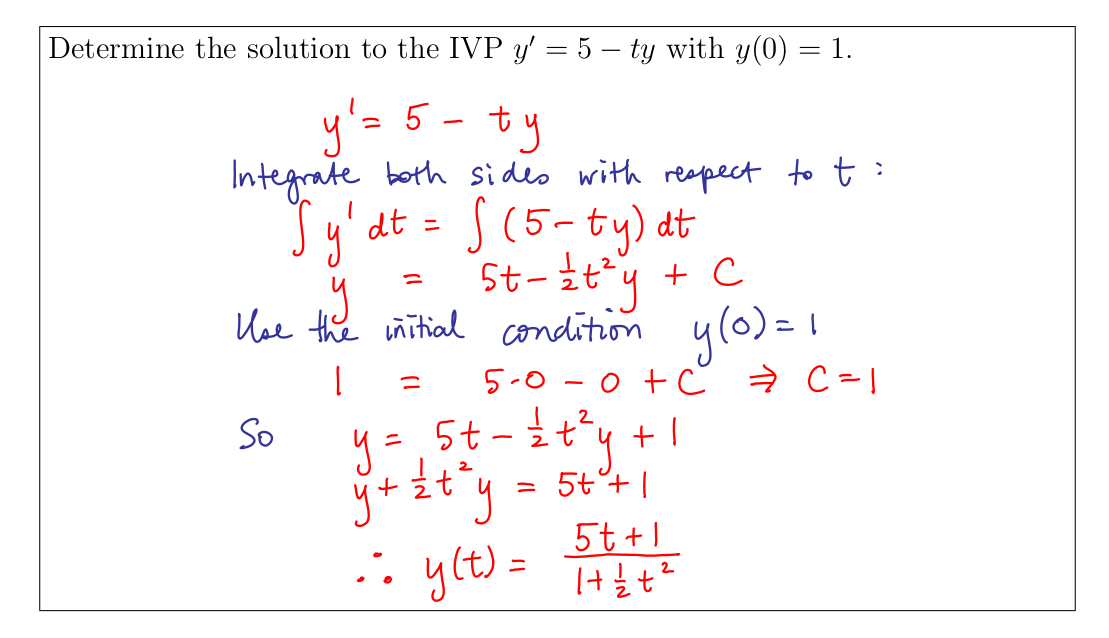
\includegraphics[scale=.4]{StudentX.png}$
\end{center}

\end{problem}
\newpage

\begin{problem}
9. You can solve $y'' = x (y')^2$ with the initial conditions $y'(0) = -2$ and $y(0) = 0$, using a change of variables combined with separation of variables. This simple example illustrates a technique that can be applied to harder problems. Here’s the idea:
\begin{itemize}
  \item First define a new variable, $w = y'$
  \item Rewrite the original DE in terms of $w$ to get a separable ODE.
  \item Solve this equation to find $w(x)$ (Note: You may want to use one of the initial condition
at this point).
  \item Substitute the answer you get for $w(x)$ into $w = y'$ and solve for $y$.
  \item Show that your solution satisfies the original DE and initial conditions.
\end{itemize}
\end{problem}
\newpage

\begin{problem}
10. Choose a topic of your liking, and find a journal article that models something in your topic
with ODEs. Once you find an article, describe the situation that is modeled in the paper.
You can use any method you like to look for articles, but we recommend using Google Scholar
(\url{https://scholar.google.com/}). Please provide the following information for the article that
you found:
 \begin{enumerate}
     \item[(a)] The title, authors, and journal in which the article appears.
     \item[(b)] A description of the DE(s). This should consist of a description of which variables are
dependent and independent variables, what the variables represent, and classification
of the ODE between linear and non-linear, autonomous and non-autonomous, and the
order of the DE.
 \end{enumerate}

If your first topic doesn’t produce any results, then try at least two other topics. For example,
we were successful using the search terms “Pilates differential equations”.

\end{problem}
\newpage
% Add pairs of problems and solutions as needed

\end{document}

